
% \section{Vorticity and Potential Vorticity}
\begin{frame}{Was ist Vortizität?}
	\begin{columns}
		\column{0.99\textwidth}
		\begin{itemize}
			\item \textbf{Vortizität} beschreibt die lokale Rotation in einer Strömung.
			\item Definiert als das \textbf{Rotationsfeld} des Geschwindigkeitsvektors:
			      \[
				      \vec{\zeta} = \nabla \times \vec{u}
			      \]
			\item Für eine zweidimensionale Strömung \( \vec{u} = (u(x,y), v(x,y)) \) ist nur die \(z\)-Komponente relevant:
			      \[
				      \zeta = \frac{\partial v}{\partial x} - \frac{\partial u}{\partial y}
			      \]
			\item \(\zeta > 0\): Zyklonale Rotation (gegen den Uhrzeigersinn)
			\item \(\zeta < 0\): Antizyklonale Rotation (im Uhrzeigersinn)
		\end{itemize}

		\column{0.4\textwidth}
		\vspace{2cm}  % Optional für vertikale Ausrichtung
	\end{columns}
\end{frame}


\begin{frame}{Zero Vorticity (Uniform Flow)}
	\begin{columns}
		\column{0.5\textwidth}
		\begin{itemize}
			\item \( \vec{u} = (2, 0) \)
			\item Uniform horizontal flow
			\item No shear or curvature
			\item \( \zeta = 0 \)
		\end{itemize}

		\column{0.5\textwidth}
		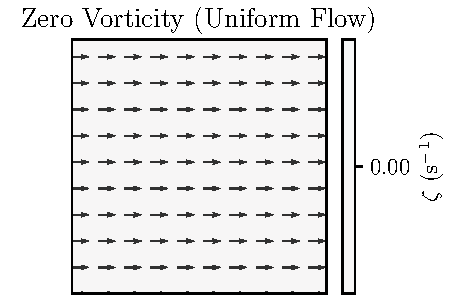
\includegraphics[width=\linewidth]{../images/vorticity_plot0.pdf}
	\end{columns}
\end{frame}

\begin{frame}{Shear Vorticity}
	\begin{columns}
		\column{0.5\textwidth}
		\begin{itemize}
			\item \( \vec{u} = (y, 0) \)
			\item Horizontal shear: \( \frac{\partial u}{\partial y} = 1 \)
			\item \( \zeta = -1 \)
		\end{itemize}

		\column{0.5\textwidth}
		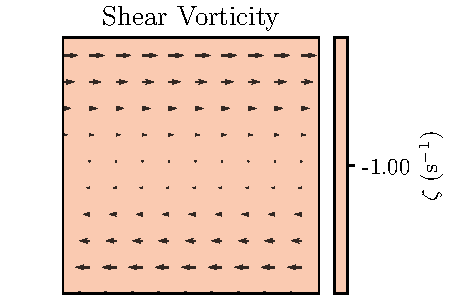
\includegraphics[width=\linewidth]{../images/vorticity_plot1.pdf}
	\end{columns}
\end{frame}

\begin{frame}{Nonlinear Shear Vorticity}
	\begin{columns}
		\column{0.5\textwidth}
		\begin{itemize}
			\item \( \vec{u} = (y^2, 0) \)
			\item \( \zeta = -2y \)
			\item Antisymmetric vorticity field
			\item Stronger at larger \( |y| \)
		\end{itemize}

		\column{0.5\textwidth}
		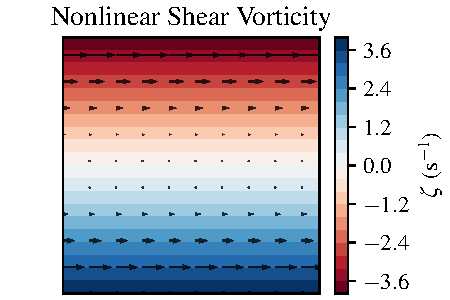
\includegraphics[width=\linewidth]{../images/vorticity_plot2.pdf}
	\end{columns}
\end{frame}

\begin{frame}{Positive Vorticity (Cyclonic)}
	\begin{columns}
		\column{0.5\textwidth}
		\begin{itemize}
			\item \( \vec{u} = (-y, x) \)
			\item Pure rotation, counter-clockwise
			\item \( \zeta = 2 \)
		\end{itemize}

		\column{0.5\textwidth}
		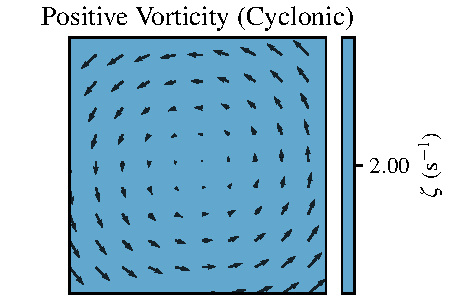
\includegraphics[width=\linewidth]{../images/vorticity_plot3.pdf}
	\end{columns}
\end{frame}

\begin{frame}{Negative Vorticity (Anticyclonic)}
	\begin{columns}
		\column{0.5\textwidth}
		\begin{itemize}
			\item \( \vec{u} = (y, -x) \)
			\item Clockwise rotation
			\item \( \zeta = -2 \)
		\end{itemize}

		\column{0.5\textwidth}
		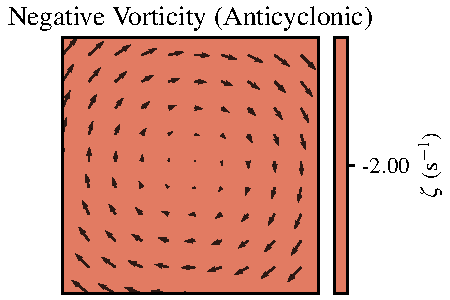
\includegraphics[width=\linewidth]{../images/vorticity_plot4.pdf}
	\end{columns}
\end{frame}

\begin{frame}{Absolute Vortizität}
  \begin{columns}
    \column{0.99\textwidth}
    \begin{itemize}
      \item In einem rotierenden Bezugssystem (wie der Erde) ergibt sich die \textbf{absolute Vortizität} zu:
      \[
        \eta = f + \zeta
      \]
      \item \( \zeta \): relative Vortizität (durch Scherung und Krümmung der Strömung)
      \item \( f = 2\Omega \sin\phi \): Coriolis-Parameter, abhängig von der geografischen Breite
      \item Bedeutend für großräumige geophysikalische Strömungen (z.\,B. Rossby-Wellen, Erhaltung der potenziellen Vortizität)
    \end{itemize}

    \column{0.4\textwidth}
    \vspace{2cm}
  \end{columns}
\end{frame}


\begin{frame}{Konservierung der potentiellen Vortizität}
  \begin{columns}
    \column{0.99\textwidth}
    \begin{itemize}
      \item Die \textbf{potenzielle Vortizität (PV)} ist definiert als:
      \[
        q = \frac{\eta}{H} = \frac{f + \zeta}{H}
      \]
      \item \( \eta \): absolute Vortizität, bestehend aus \( f + \zeta \)
      \item \( H \): effektive Schichtdicke (z.\,B. Troposphärenhöhe oder isentrope Dicke)
      \item In einer reibungsfreien, adiabatischen Atmosphäre gilt:
      \[
        \frac{Dq}{Dt} = 0
      \]
      \item \textbf{Folge:} PV ist entlang von Teilchenbahnen erhalten → zentrale Größe in der großskaligen Dynamik
    \end{itemize}

    \column{0.4\textwidth}
    \vspace{2cm}
  \end{columns}
\end{frame}



% \begin{frame}{Barotrope Vorticity-Gleichung}
%     \begin{itemize}
%       \item Annahmen:
%       \begin{itemize}
%         \item Nicht-divergente Strömung
%         \item Eine Schicht (barotropes Modell)
%       \end{itemize}
%       \item Vorticity-Gleichung (mit \(\psi\): Stromfunktion):
%       \[
%         \frac{\partial}{\partial t}(\nabla^2 \psi) + \beta \frac{\partial \psi}{\partial x} = 0
%       \]
%       \item Wellenlösung: 
%       \[
%         \psi = \Re \left\{ \hat{\psi} \, e^{i(kx + ly - \omega t)} \right\}
%       \]
%       \item Dispersionsrelation:
%       \[
%         \omega = -\beta \frac{k}{k^2 + l^2}
%       \]
%       \item \textbf{Folgen}:
%       \begin{itemize}
%         \item Westwärts laufende Rossby-Wellen (\( \omega < 0 \) für \( k > 0 \))
%         \item Phasengeschwindigkeit \( \neq \) Gruppengeschwindigkeit
%       \end{itemize}
%     \end{itemize}
%     \end{frame}
